\let\negmedspace\undefined
\let\negthickspace\undefined
\documentclass[journal]{IEEEtran}
\usepackage[a5paper, margin=10mm, onecolumn]{geometry}
\usepackage{tfrupee} % Include tfrupee package

\setlength{\headheight}{1cm} 
\setlength{\headsep}{0mm}     

\usepackage{gvv-book}
\usepackage{gvv}
\usepackage{cite}
\usepackage{amsmath,amssymb,amsfonts,amsthm}
\usepackage{algorithmic}
\usepackage{graphicx}
\usepackage{textcomp}
\usepackage{xcolor}
\usepackage{txfonts}
\usepackage{listings}
\usepackage{enumitem}
\usepackage{mathtools}
\usepackage{gensymb}
\usepackage{comment}
\usepackage[breaklinks=true]{hyperref}
\usepackage{tkz-euclide} 
\usepackage{listings}
\def\inputGnumericTable{}                                 
\usepackage[latin1]{inputenc}                                
\usepackage{color}                                            
\usepackage{array}                                            
\usepackage{longtable}                                       
\usepackage{calc}                                             
\usepackage{multirow}                                         
\usepackage{hhline}                                           
\usepackage{ifthen}                                           
\usepackage{lscape}
\usepackage{circuitikz}
\tikzstyle{block} = [rectangle, draw, fill=blue!20, 
    text width=4em, text centered, rounded corners, minimum height=3em]
\tikzstyle{sum} = [draw, fill=blue!10, circle, minimum size=1cm, node distance=1.5cm]
\tikzstyle{input} = [coordinate]
\tikzstyle{output} = [coordinate]


\begin{document}

\bibliographystyle{IEEEtran}
\vspace{3cm}

\title{4.13.1}
\author{AI25BTECH11036-SNEHAMRUDULA}
 \maketitle
{\let\newpage\relax\maketitle}
\renewcommand{\thefigure}{\theenumi}
\renewcommand{\thetable}{\theenumi}
\setlength{\intextsep}{10pt} 
\numberwithin{equation}{enumi}
\numberwithin{figure}{enumi}
\renewcommand{\thetable}{\theenumi}
\textbf{Question}:\\

Consider the lines given by
\begin{align*}
L_1 &: x + 3y - 5 = 0, \\
L_2 &: 3x - ky - 1 = 0, \\
L_3 &: 5x + 2y - 12 = 0.
\end{align*}
Match the Statements/Expressions in Column I with the Statements/Expressions in Column II.

\begin{center}
\begin{tabular}{p{0.45\linewidth} p{0.45\linewidth}}
\textbf{Column I} & \textbf{Column II} \\
\begin{enumerate}[label=(\Alph*)]
    \item $L_1, L_2, L_3$ are concurrent, if
    \item One of $L_1, L_2, L_3$ is parallel to at least one of the other two, if
    \item $L_1, L_2, L_3$ form a triangle, if
    \item $L_1, L_2, L_3$ do not form a triangle, if
\end{enumerate}
&
\begin{enumerate}[label=(\alph*)]
    \item $k = 9$
    \item $k = \dfrac{-6}{5}$
    \item $k = \dfrac{5}{6}$
    \item $k = 5$
\end{enumerate}
\end{tabular}
\end{center}
\textbf{Solution.}
cc
\begin{frame}{Graphical Representation}
\begin{center}
% placeholder figure drawn with TikZ
\begin{tikzpicture}[scale=0.7]
  % Axes
  \draw[->] (-1,0)--(5,0) node[right]{$x$};
  \draw[->] (0,-1)--(0,4) node[above]{$y$};

  % Lines
  \draw[red, thick] (-1,2) -- (5,0.0) node[right] {$L_1$};
  \draw[blue, thick] (-1,-1) -- (4,5) node[right] {$L_2$};
  \draw[green!70!black, thick] (-1,4.25) -- (4,1) node[right] {$L_3$};

  % Intersection point
  \fill (2,1) circle (2pt) node[below right] {$(2,1)$};
\end{tikzpicture}
\end{center}
\end{frame}

\end{document}q
